\subsection{Liquidity Rebalancing System\label{section:lrs}}

The best user experience is obtained when the liquidity availability is high thus allowing, in general, any token to be moved from any network to any other network.

To that end, we used the LSE from Sec.~\ref{section:lse} to design a forecasting and rebalancing technology which can predict in advance when a certain liquidity level will be reached for a given vault. This is built into Mosaic.
%
It is critical for the optimization of the passive liquidity rebalancing that will enable passive liquidity providers to continue to service cross-layer transfers.
%
Having an optimal allocation of capital across layers is key to offering the best performance for users seeking to move cross-layer. Therefore, understanding when said capital reaches certain key levels where action will need to be taken is important.

More formally, enter the Liquidity Rebalancing System (LRS) developed by Composable Labs.
%
\begin{figure}
    \centering
    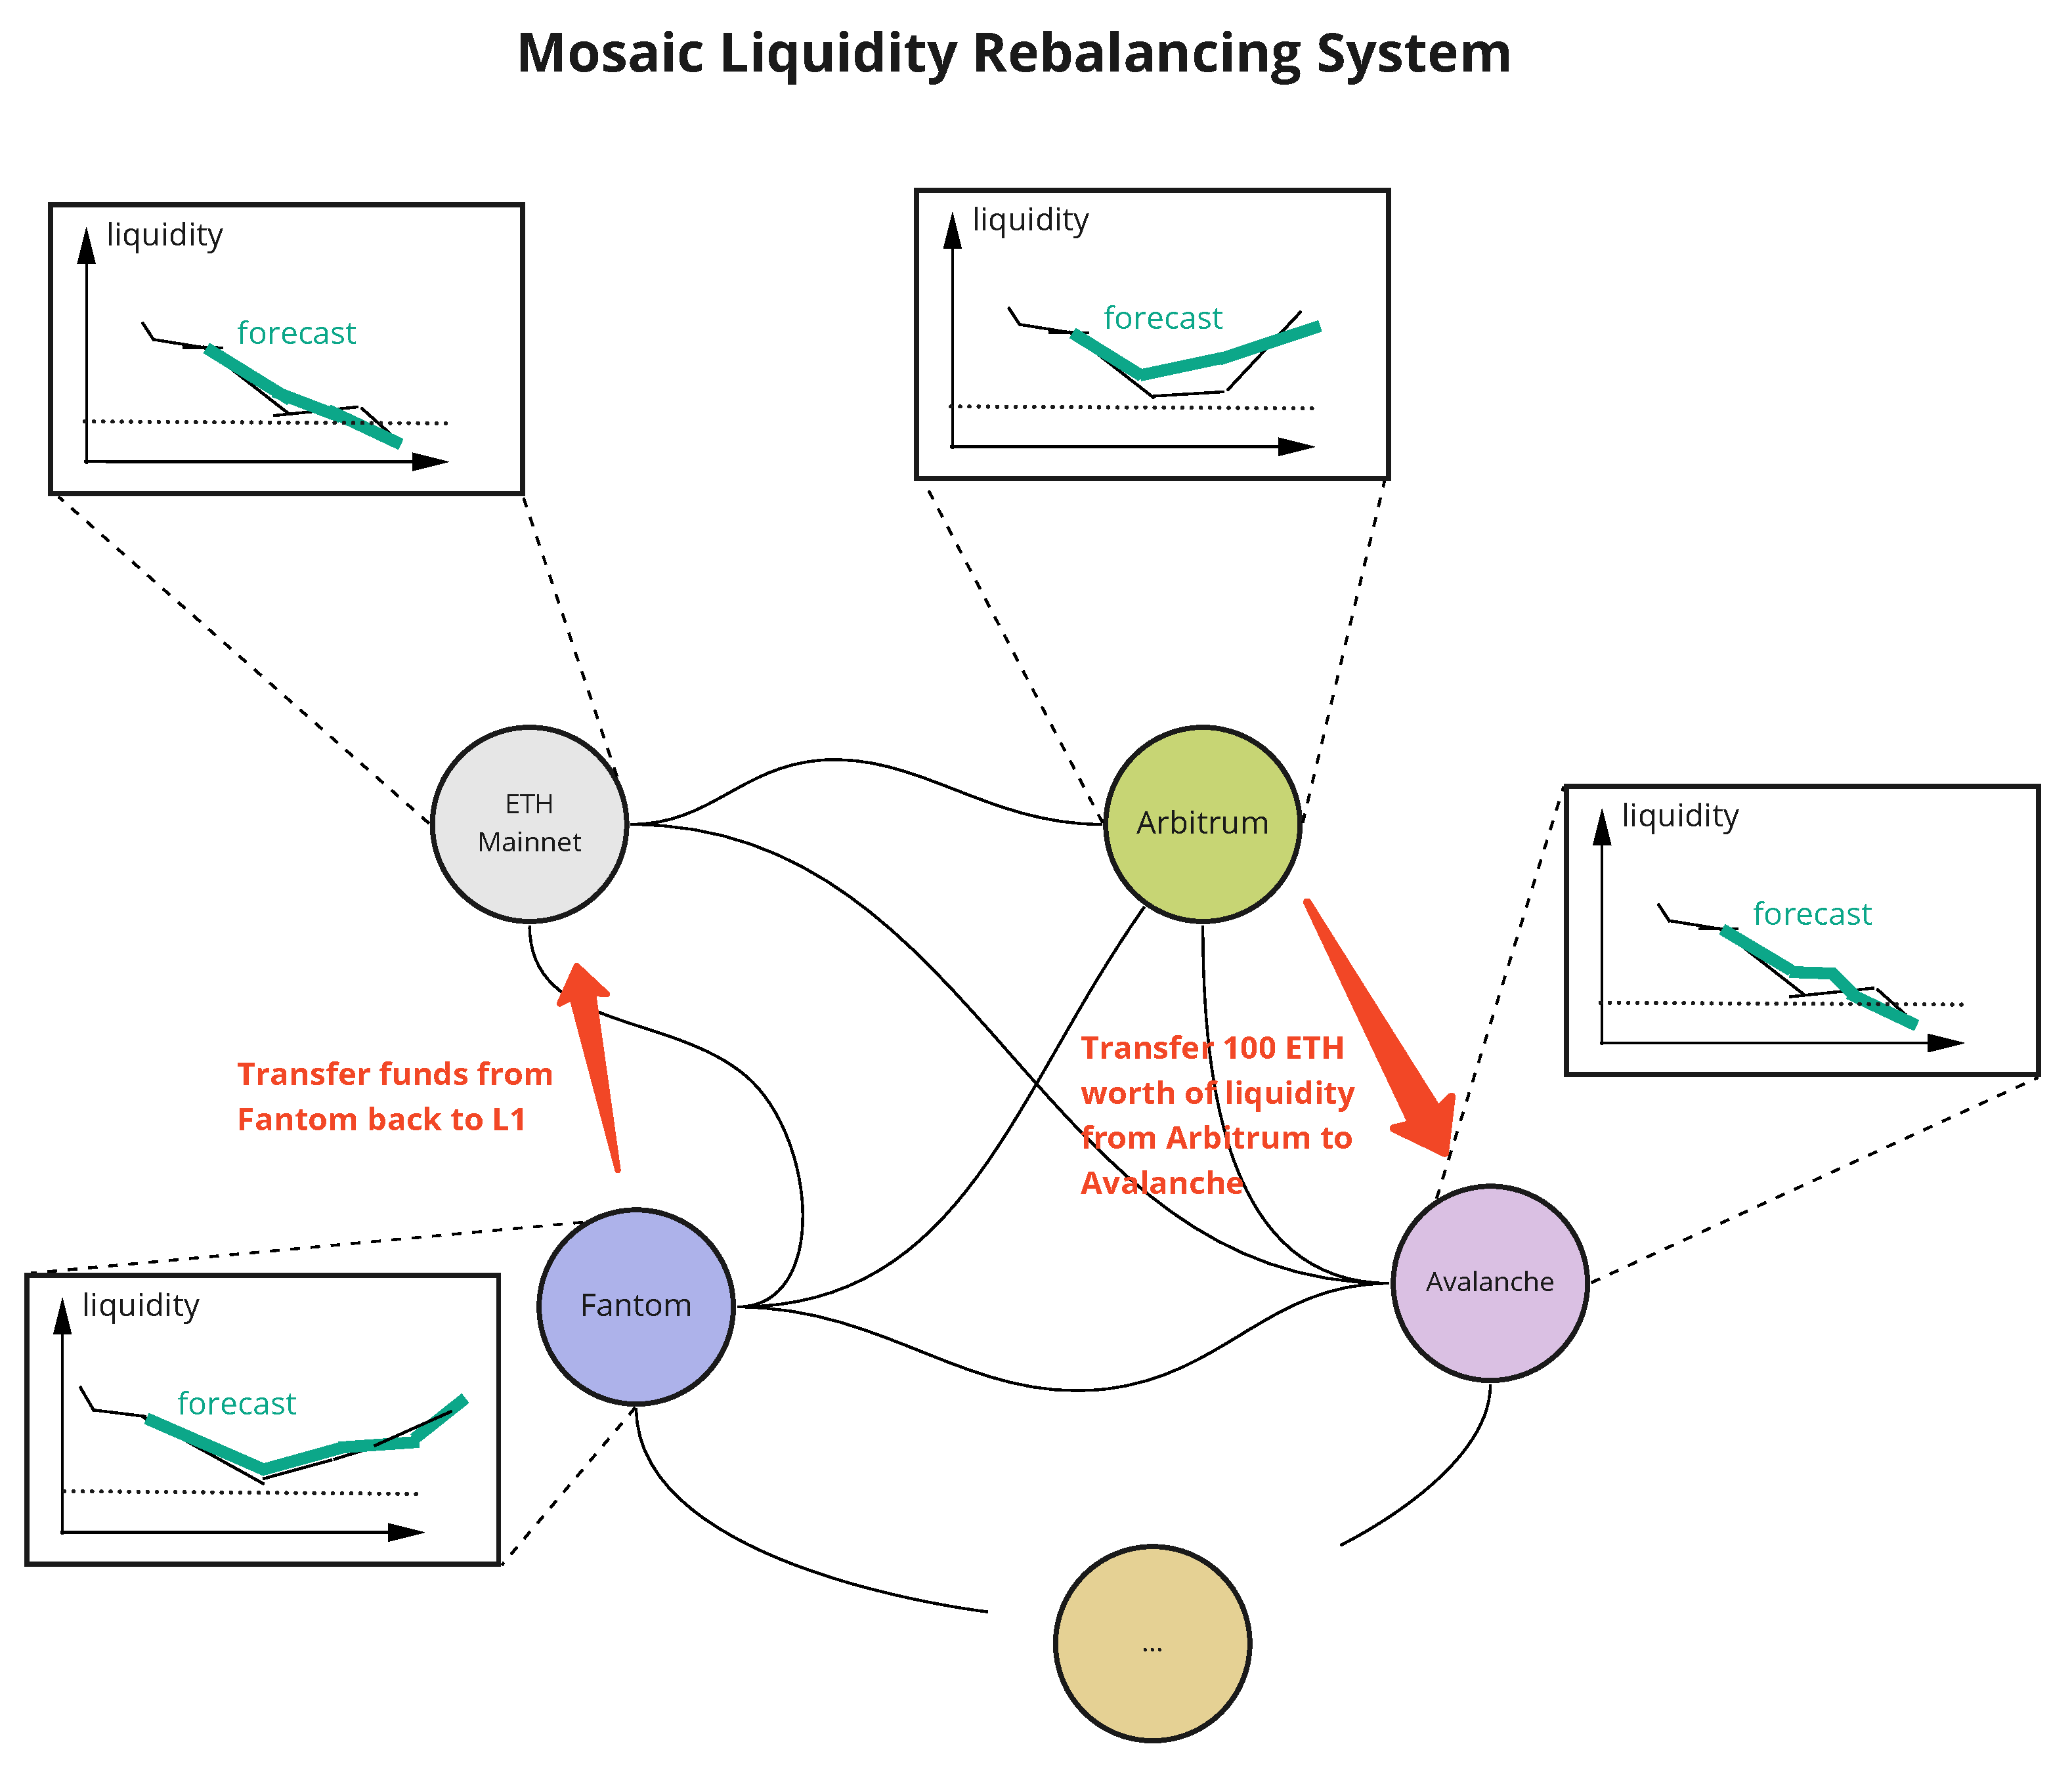
\includegraphics[scale=0.22]{images/lrs.pdf}
    \caption{Sketch of the Liquidity Rebalancing System showing how a forecast model is built on the liquidity in each vault in the Mosaic network. Transfer of funds are moved as needed when a subset of vaults are depleted (to a certain pre-set level, we use 90\% here which is conservative) needing funds from a donor vault.}
    \label{fig:lrs}
\end{figure}
%
In Fig.~(\ref{fig:lrs}) we show a graph of various networks such as the Ethereum mainnet, a layer 2 solution Arbitrum, Avalanche, and Fantom, but Mosaic supports many more networks and is growing.

LRS builds a forecasting model on each network (shown as the insets with black lines being the liquidity data and green lines being the forecast model). At a given frequency, e.g. hourly, it checks the status of all networks, computes where liquidity is needed and performs the transfers.
%
The transfers take place as follows: if a vault is predicted to be depleted to 80\% of its seed amount then funds are moved from a so-called ``donation" vault. If a vault has too much liquidity, or satisfy a broader set of metrics to be defined later, it becomes a donation vault (this status is temporary).

The system overall consists of two key pieces: First, we have a forecasting model predicting the evolution of liquidity in a single vault on a single network and second, we have a broader logic deciding how to distribute available liquidity across the entire connection of networks (a connected graph).

\subsubsection{Forecasting a Single Network}

To forecast a single network we developed multiple models starting with a set of baseline models including an autoregressive integrated moving average (ARIMA) model \cite{AnScience}, Holt's linear trend model (HLT) \cite{7.2Ed}, and a Holt-Winters seasonal method \cite{7.3Ed}. We will show the ARIMA and HLT performance in what follows.

Also, the eventual goal is to build Artificial Intelligence (AI) \cite{ArtificialBritannica} based models such as long short-term memory (LSTM) \cite{UnderstandingBlog}.
%
This work is in the pipeline and the non-AI baseline models will help us compare and also develop a two-tiered system where non-AI and AI work to forecast together.

\subsubsection*{Forecasting with ARIMA}

To simplify the discussion and without loss of generality we assume a graph of three networks: L1, Arbitrum (ARB), and Polygon (POL).
%
We first develop an ARIMA model to fit and forecast liquidity data on the POL vault, that can be mathematically described as 
%
\begin{equation}
    Y_t - \alpha_1Y_{t-1} - \dots - \alpha_{p'}Y_{t-p'} = \epsilon_t + \theta_1\epsilon_{t-1} + \dots + \theta_q\epsilon_{t-q},
\end{equation}
%
where $Y_t$ is our time series data at discrete time $t$. Although the above expression applies to the more widely known \emph{autoregressive moving average} (ARMA) \cite{TimeScience} models with $p'$ and $q$ being the orders of the autoregressive (AR) and moving average (MA) terms, here we also account for the fact that non-stationary effects are present in our data and, therefore, a differencing step needs to be applied to the data prior to fitting the model.
%
The order of the differencing step depends on the multiplicity of the unit root. Using the lag operator notation, $L^i[Y_t] := Y_{t-i}$, the times series model can be written as 
%
\begin{equation}
    \left(1 - \sum_{i=1}^{p'} \alpha_i L^i\right) Y_t = \left(1 + \sum_{i=1}^p\theta_i L^i\right)\epsilon_t
\end{equation}
%
and in the presence of a unit root with multiplicity $d$ we have 
%
\begin{equation}
    \left(1 - \sum_{i=1}^{p} \phi_i L^i\right) (1 - L)^d Y_t = \delta + \left(1 + \sum_{i=1}^p\theta_i L^i\right)\epsilon_t
\end{equation}
%
representing the ARIMA(p, d, q) process.

Next, we developed an automated model selection of the ARIMA order parameters such that the rebalancing system does not require manual input to determine its parameters when a dataset is provided.
%
Below we are presenting a list of criteria that we have used in order to identify the optimal order of differencing $d$ in the data and the orders of autoregressive and moving average terms, $p$ and $q$, in the ARIMA(p, d, q) model. 

\subsubsection*{Identifying the order of differencing in the data}

The first step in fitting an ARIMA model is the determination of the order of differencing needed to ``stationarize" the series. Normally, the correct amount of differencing is the lowest order of differencing that yields a time series which fluctuates around a well-defined mean value and whose autocorrelation function (ACF) plot decays fairly rapidly to zero, either from above or below. If the series still exhibits a long-term trend, or otherwise lacks a tendency to return to its mean value, or if its autocorrelations are positive out to a high number of lags (e.g., 10 or more), then it needs a higher order of differencing. Although the presence of most of these characteristics can be observed by simply looking at the differenced data plots, in order to automate our model selection procedure, we work primarily with the autocorrelation function.

The first rule that we apply is that, if the series has positive autocorrelations out to a high number of lags, then we increase the order of differencing by one. 
A sign that can often indicate that the time series might be overdifferenced is to observe an lag-1 autocorrelation that is below $-0.5$. In practice, in order to apply these two rules, we fit an ARIMA(0, d, 0) model, that is a model with no AR or MA terms, but only a constant term which when trained, it provides an estimate of the mean of the data. Thus, the residuals of this model is simply the deviation from the mean. Once we identify a sufficient $d$ such that the aurocorrelation function drops to small values past lag-1, we also compare the resulting model with an ARIMA(0, d+1, 0). Assuming that lag-1 autocorrelation does not fall below $-0.5$ (which would be a sign of overdifferencing), if the model with d+1 order of differencing exhibits lower standard deviation values then it is preferred over $d$, otherwise we keep $d$ and we proceed with the selection of optimal $p$ and $q$ orders. 

\subsubsection*{Identifying the AR(p) and MA(q) orders}

Next, in order to identify the number of autoregressive and moving average terms, we proceed as follows: 
For the number $p$ of AR terms we set it equal to the number of lag terms that it takes for the partial autocorrelation function (PACF) to cross the significance limit.
%
Similarly, the number $q$ of MA terms, we use the autocorrelation function (ACF) instead and it is set again equal to the number of lag terms that it takes to cross the significance limit. 

\subsubsection*{Optimizing the ARIMA model for our LSE data}

In what follows we employ our model selection capability explained above to optimize our ARIMA model parameters and use them for forecasting.

We generate simulated data with the LSE. Our time series data consists of $1000$ liquidity transfer observations obtained on a hourly basis ($\Delta t = 1$ hour).
%
We briefly touched on how these are computed, but let us provide more details here. We select a number of token movements of the vaults. These are drawn from a truncated Gaussian with parameters set to resemble real-world transfers. As an aside, the Mosaic PoC provided even more realistic data and we have developed ways to account for this as well - we are able to confirm that our simulated data resembles the PoC data.
%
Then, the simulated data is snapped to a global timegrid and a state machine is used to evolve the vault states forward starting at some initial liquidity levels. This give rise to the evolving liquidity levels over time as plotted in Fig.~(\ref{fig:lse_datasets}).

\begin{figure}
    \centering
    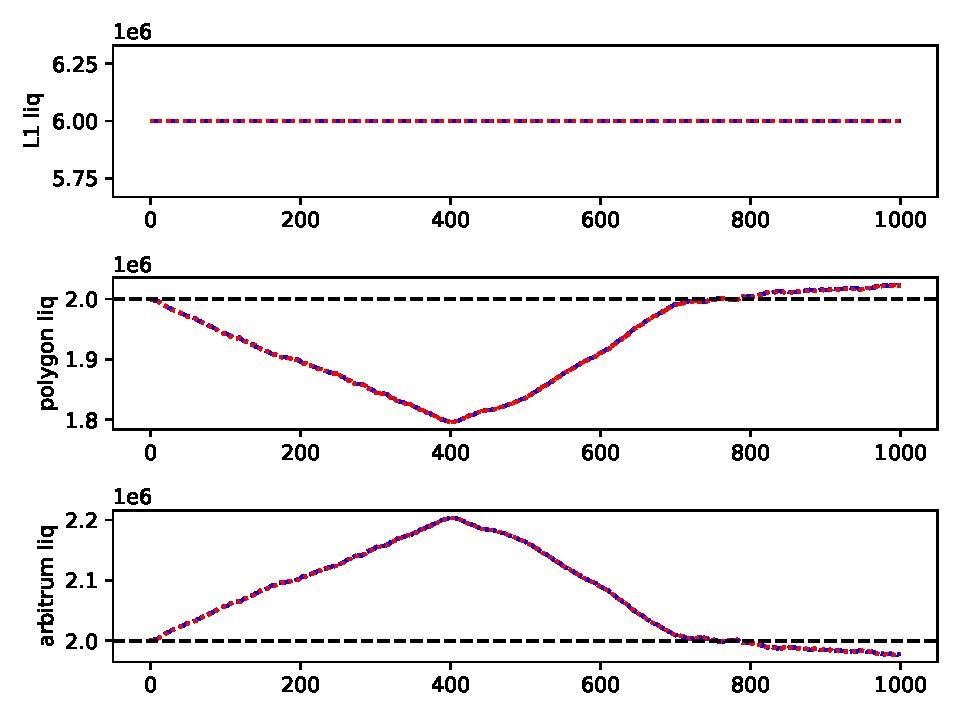
\includegraphics[width=0.49\textwidth]{images/lse_results_feemodel_3_20_20211015_18_59_40_412997.pdf}
    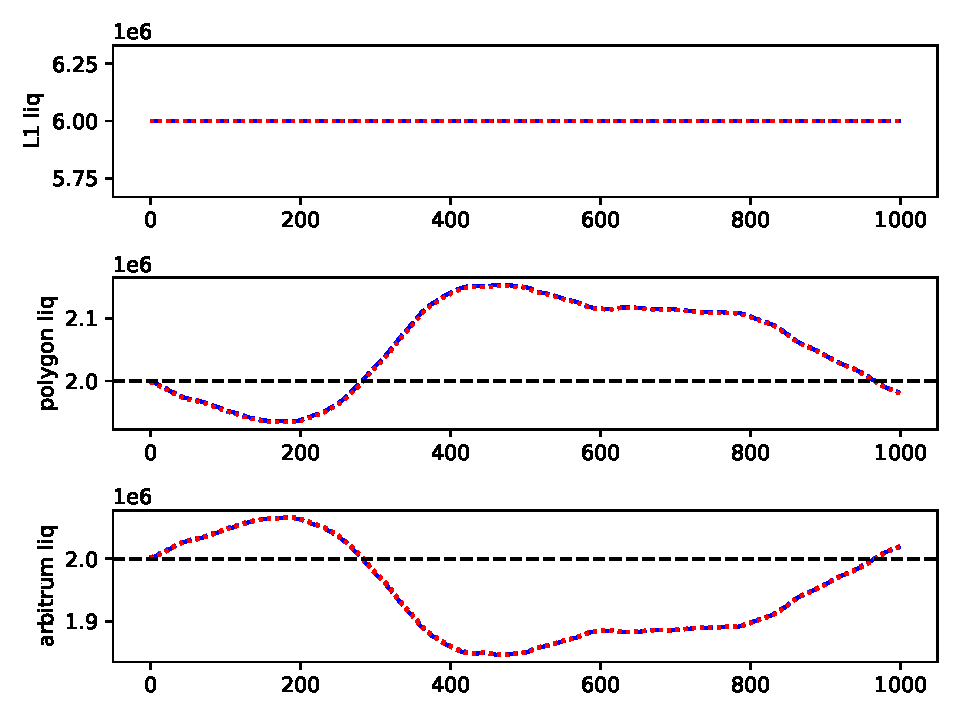
\includegraphics[width=0.49\textwidth]{images/lse_results_feemodel_3_20_20211021_18_59_52_314364.pdf}
    \caption{Dataset 1 (left) and Dataset 2 (right) from the Liquidity Simulation Environment (LSE). Each vault is a row. The liquidity is shown as the moving curves in rows 2 and 3. Row 1 does not have transfers involved with it for this data.}
    \label{fig:lse_datasets}
\end{figure}

We use $200$ training points (roughly 8 days worth of data) each time we fit an ARIMA model and we use it to forecast on a time horizon of $168$ hours; roughly 1 week ahead which coincides with some layer 2 to layer 1 exit times.

Then, we run the model selection algorithm every time we shift the time frame 10 time steps ahead, and we find that in all cases the number of AR terms varies from $3$ to $6$ while the optimal number of MA terms is always $1$ for both Datasets 1 and 2.

We next show the performance of the ARIMA model as well as of HLT. In the HLT approach, also known as double exponential smoothing, we identify a linear trend in the time series and make a prediction using the smoothed value $s_t$ and the linear trend term $b_t$ at time $t$.

See the forecasting comparison and performance for the Arbitrum vault in Fig.~(\ref{fig:arb_conserv}).

\begin{figure}[h]
    \centering
    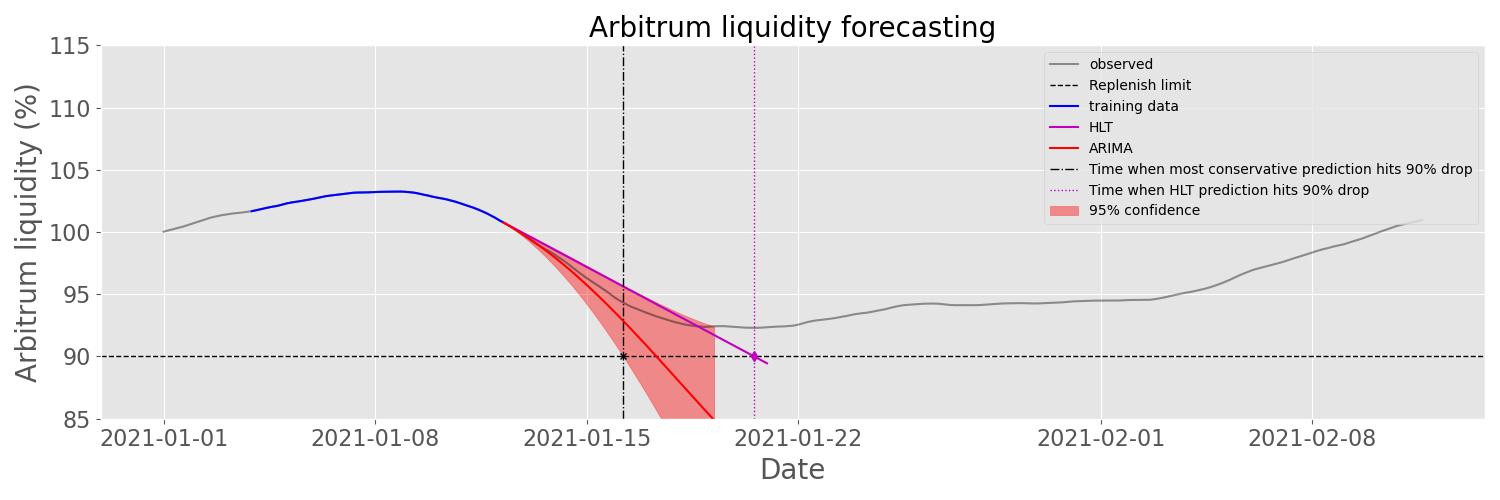
\includegraphics[width=\textwidth]{images/arbitrum_instance_t_fin270_90perce_drop.png}
    \caption{Forecasting comparison between ARIMA and HLT models. The black point shows when the ARIMA model predicts that a 90\% liquidity level is reached in the vault - by conservative estimates (the lower confidence level). The purple point shows when the HLT model predicts the same 90\% liquidity level. While both predictions can be used to trigger, in advance, a replenishment event, the ARIMA predictions appears to be much more conservative.}
    \label{fig:arb_conserv}
\end{figure}

We run a forecasting model on each vault and this, in turn, triggers the rebalancing system to move liquidity accordingly to always keep the vaults ready and liquid thus maximizing the successful transfer rate.

We note that, as we run the forecasting model across the data in a rolling window fashion, the data is contained within the 95\% confidence bands in the amount of time expected allowing us to perform accurate and conservative replenishment event estimates.

\subsubsection{Rebalancing Logic}

With a forecasting model built on each network, the next step is designing the rebalancing logic of the overall system.
%
Here is our approach. At a given cadence which can depend on transfer activity in the general network, we check the following: First, what is the set of current liquidity donation vault. We assign a score to each vault and sort them. For each donor, we also log how much liquidity can be donated.
%
This implies that we have a list of candidate liquidity donors.
%
Next, we obtain the list of vaults which are in need of liquidity. Perhaps this is an empty set, but assuming not, we simply deplete as much liquidity from the donors going top down until all liquidity has been rebalanced.

The score assigned to a vault in the ``donor detection phase" is determined based on a set of metrics including: how active is this vault (inactive implies that it can donate without needing liquidity itself), how much ``active" liquidity is assigned vs passive, what value the forecasting model predicts it will take in the future (is it generally increasing or decreasing in liquidity), and many more.
